\documentclass[11pt,a4paper]{article}

\usepackage[utf8]{inputenc}
\usepackage[T1]{fontenc}
\usepackage{lmodern}
\usepackage[margin=1in]{geometry}
\usepackage{amsmath,amssymb}
\usepackage{graphicx}
\usepackage{booktabs}
\usepackage{hyperref}
\usepackage{cleveref}
\usepackage{xcolor}
\usepackage{listings}
\usepackage{enumitem}
\usepackage{tikz}
\usetikzlibrary{shapes.geometric,arrows.meta,positioning,fit,calc}
\usepackage{pgfplots}
\pgfplotsset{compat=1.18}
\usepackage{caption}
\usepackage{multirow}
\usepackage{makecell}
\usepackage{natbib}
\usepackage{mdframed}
\usepackage{tcolorbox}
\tcbuselibrary{listings,breakable,skins}

\hypersetup{
  colorlinks=true,
  linkcolor=blue!70!black,
  citecolor=green!50!black,
  urlcolor=blue!60!black,
}

% ── Code listings ────────────────────────────────────────────────────
\lstdefinestyle{shell}{
  basicstyle=\ttfamily\small,
  backgroundcolor=\color{gray!10},
  frame=single,
  framerule=0.4pt,
  breaklines=true,
  columns=fullflexible,
  keepspaces=true,
  upquote=true,
}
\lstdefinestyle{python}{
  language=Python,
  basicstyle=\ttfamily\small,
  backgroundcolor=\color{blue!5},
  frame=single,
  framerule=0.4pt,
  keywordstyle=\color{blue!70!black}\bfseries,
  commentstyle=\color{green!50!black},
  stringstyle=\color{red!60!black},
  breaklines=true,
  columns=fullflexible,
  keepspaces=true,
}
\lstdefinestyle{output}{
  basicstyle=\ttfamily\footnotesize,
  backgroundcolor=\color{black!5},
  frame=single,
  framerule=0.4pt,
  breaklines=true,
  columns=fullflexible,
  keepspaces=true,
}

% ── Callout boxes ────────────────────────────────────────────────────
\newtcolorbox{keyinsight}[1][]{
  colback=blue!5!white, colframe=blue!60!black,
  fonttitle=\bfseries, title=Key Insight,
  breakable, #1
}
\newtcolorbox{warning}[1][]{
  colback=orange!8!white, colframe=orange!70!black,
  fonttitle=\bfseries, title=Warning,
  breakable, #1
}
\newtcolorbox{casestudy}[2][]{
  colback=green!5!white, colframe=green!50!black,
  fonttitle=\bfseries, title=Case Study #2,
  breakable, #1
}

% ── Notation ─────────────────────────────────────────────────────────
\newcommand{\Bshort}{B_{\text{short}}}
\newcommand{\Ps}{\mathcal{P}_s}
\newcommand{\Pl}{\mathcal{P}_l}

% ====================================================================
\title{%
  \texttt{inference-fleet-sim}\\[4pt]
  \large A Practitioner's Guide to LLM GPU Fleet Simulation:\\
  Education, Usage, and Case Studies%
}

\date{2026}

\begin{document}
\maketitle
\tableofcontents
\newpage

% ====================================================================
\section{Who Should Read This Guide}
\label{sec:intro}

This guide is for \textbf{ML platform engineers, capacity planners, and
researchers} who need to answer questions such as:

\begin{itemize}[nosep]
  \item \textit{``How many A100 GPUs do I need to serve 300 requests/s
    at P99 TTFT $\leq$ 500\,ms?''}
  \item \textit{``If my traffic doubles next quarter, when will I
    breach my SLO and by how much?''}
  \item \textit{``Should I run one homogeneous GPU fleet or split into
    short- and long-context pools?''}
  \item \textit{``My fleet is sized for today's workload. How much
    does Compress-and-Route (C\&R) help?''}
  \item \textit{``Which routing algorithm minimises tail latency for
    my agent-heavy traffic?''}
\end{itemize}

\texttt{inference-fleet-sim} is a \textbf{fleet-level discrete-event
simulator} for LLM inference.  Unlike single-instance simulators such
it models the full picture: multiple GPU pools, heterogeneous hardware,
pluggable routing algorithms, and an analytical optimizer that finds the
minimum-cost fleet meeting a P99 TTFT SLO.

\paragraph{Prior art and scope.}
Single-instance simulators (e.g., Vidur~\citep{vidur2024},
vLLM offline profilers) are invaluable for engine-level tuning ---
understanding KV-cache block utilization, preemption rates, and
chunked-prefill scheduling.  This tool is complementary: it operates
one abstraction level higher, modeling the fleet as a network of M/G/$c$
queues and asking how many GPUs are needed, how they should be grouped
into pools, and which routing policy minimises tail latency.

\paragraph{What this guide covers.}
Section~\ref{sec:background} explains the underlying concepts (queueing
theory, the cost cliff, TTFT decomposition) at a practitioner level.
Section~\ref{sec:architecture} describes the simulator's internals.
Section~\ref{sec:quickstart} is a 5-minute quick start.
Section~\ref{sec:cli} documents every CLI command.
Section~\ref{sec:casestudies} walks through four real-world case
studies with full command output.
Section~\ref{sec:extend} explains how to extend the simulator.

% ====================================================================
\section{Background: Key Concepts}
\label{sec:background}

\subsection{Why GPU Fleets Are Expensive to Get Right}

Modern LLMs support context windows up to 128K tokens, but production
traces tell a different story: in the Azure LLM Inference Trace, $\sim$78\%
of requests use fewer than 2K tokens (CDF value $F(2{,}048) \approx 0.78$).  A fleet provisioned for
worst-case context length allocates KV-cache memory that sits idle
for nearly every request.

The cost of this mismatch is not gradual.  The simulator models KV-cache
capacity via PagedAttention blocks: each A100-80GB holds
\texttt{total\_kv\_blks=65\,536} blocks of \texttt{blk\_size=16} tokens.
A sequence using up to 64K tokens needs $\lceil 65{,}536/16 \rceil = 4{,}096$
blocks, so only $\lfloor 65{,}536 / 4{,}096 \rfloor = \mathbf{16}$ sequences
fit concurrently.  The same GPU at an 8K context boundary needs only
$\lceil 8{,}192/16 \rceil = 512$ blocks per sequence, allowing
$\lfloor 65{,}536 / 512 \rfloor = \mathbf{128}$ concurrent sequences ---
an \textbf{8$\times$ throughput difference} between the two pool types.

\subsection{Pool Routing and the Cost Cliff}
\label{sec:bg-routing}

\textbf{Pool routing} splits the fleet into two pools:
\begin{itemize}[nosep]
  \item \textbf{Short pool} $\Ps$: sized for $\Bshort$ tokens (e.g., 8K),
    128 concurrent sequences per GPU.
  \item \textbf{Long pool} $\Pl$: sized for full context (e.g., 64K),
    16 concurrent sequences per GPU.
\end{itemize}
Each request is routed to $\Ps$ if its estimated total token budget
$L_{\text{total}} \leq \Bshort$, else to $\Pl$.  This saves 16--38\%
of GPU cost versus a homogeneous fleet.

The \textbf{cost cliff} is the discontinuity at $\Bshort$: a request
at $\Bshort + 1$ tokens occupies one of only 16 long-pool slots,
consuming $8\times$ more throughput capacity than its immediate
neighbour below $\Bshort$.  Requests in the \emph{borderline band}
$(\Bshort,\, \gamma\Bshort]$ are not genuinely long; they just barely
crossed the threshold.  Compress-and-Route (C\&R) addresses this by
compressing borderline prompts back below $\Bshort$ at the gateway.

\subsection{The M/G/c Queue: Explaining the Math Behind GPU Sizing}
\label{sec:mgc}

The simulator's analytical core models each GPU pool as an
\textbf{M/G/$c$ queue}:

\begin{center}
\begin{tabular}{clp{9cm}}
\toprule
Letter & Stands for & Meaning in our context \\
\midrule
\textbf{M} & Markovian arrivals & Requests arrive as a Poisson process with
  rate $\lambda$; each arrival is independent \\
\textbf{G} & General service & Each request takes a different amount of GPU time;
  captured by mean $\mathbb{E}[S]$ and variance $\mathrm{Var}[S]$ \\
\textbf{$c$} & $c$ servers & The pool has $c$ GPUs running in parallel;
  requests queue until a GPU is free \\
\bottomrule
\end{tabular}
\end{center}

\paragraph{Why ``G'' not ``M'' for service time?}
Real LLM requests vary enormously: a 50-token chat reply takes
$\sim$100\,ms; a 50K-token RAG response takes $\sim$30\,s.  Using an
exponential service distribution (M/M/$c$) would underestimate tail
latency for high-variance workloads.  The \textbf{Kimura (1994)
correction} scales the Erlang-C waiting time by $(1 + C_s^2)/2$,
where $C_s^2 = \mathrm{Var}[S]/(\mathbb{E}[S])^2$ is the squared
coefficient of variation.  A high-$C_s^2$ workload (heavy-tailed
request lengths) queues much worse than M/M/$c$ predicts.

\paragraph{The Erlang-C formula.}
Let $\varrho = \lambda/(c\mu)$ be the per-server utilization.  The
probability that an arriving request has to wait (all $c$ GPUs busy):
\begin{equation}
  C(c, \varrho) = \frac{(c\varrho)^c / (c!\,(1-\varrho))}{%
    \sum_{k=0}^{c-1}(c\varrho)^k/k! + (c\varrho)^c/(c!\,(1-\varrho))}.
  \label{eq:erlang-c}
\end{equation}
The P99 queue waiting time under the Kimura approximation:
\begin{equation}
  W_{99} \approx \frac{C(c,\varrho)}{c\mu(1-\varrho)}
    \cdot \frac{1+C_s^2}{2} \cdot \ln(100).
  \label{eq:w99}
\end{equation}

\begin{keyinsight}
  $W_{99}$ grows without bound as $\varrho \to 1$ (GPU utilization
  approaches 100\%).  At $\varrho = 0.94$, the analytical model
  predicts P99 wait $\approx$ 325\,ms.  At $\varrho = 0.97$, it
  exceeds 800\,ms.  The simulator enforces $\varrho_{\max} = 0.85$
  to stay in the regime where the approximation is accurate
  (8--14\% conservative overestimate vs.\ DES).
\end{keyinsight}

\paragraph{The service time model.}
GPU iteration latency under continuous batching scales with the number
of concurrent sequences $n_{\text{slots}}$:
\begin{equation}
  t_{\text{iter}} = W + H \cdot n_{\text{slots}},
  \label{eq:iter}
\end{equation}
where $W = 8$\,ms (baseline compute for Llama-3-70B/A100) and
$H = 0.65$\,ms/slot (memory-bandwidth cost per concurrent sequence).
A request with $L_{\text{in}}$ input tokens and $L_{\text{out}}$
output tokens has expected service time:
\begin{equation}
  \mathbb{E}[S] = \frac{\lceil L_{\text{in}} / C_{\text{chunk}} \rceil
    + L_{\text{out}}}{n_{\max}} \cdot t_{\text{iter}},
  \label{eq:service-time}
\end{equation}
where $C_{\text{chunk}}$ is the prefill chunk size (default 512) and
$n_{\max}$ is the pool's max concurrent sequences per GPU.

\subsection{TTFT Decomposition}
\label{sec:ttft}

Time-to-First-Token (TTFT) decomposes as:
\begin{equation}
  \text{TTFT} = \underbrace{W_{\text{queue}}}_{\text{wait for GPU slot}}
    + \underbrace{T_{\text{prefill}}}_{\text{process input tokens}}
    + \underbrace{t_{\text{iter}}}_{\text{first decode step}}.
\end{equation}
The SLO applies to the full TTFT, not just the queue wait.
$T_{\text{prefill}} = \lceil L_{\text{in}}/C_{\text{chunk}}\rceil
\cdot t_{\text{iter}}$ is the wall-clock prefill time (independent of
batch size since all slots run in parallel each iteration).

\begin{warning}
  For large requests near $\Bshort$, $T_{\text{prefill}}$ alone can
  exceed 100\,ms.  At $L_{\text{in}} = 8{,}192$ tokens with
  $C_{\text{chunk}} = 512$: $\lceil 8{,}192/512 \rceil = 16$
  iterations $\times$ 8\,ms = 128\,ms prefill, leaving only 372\,ms
  for queueing under a 500\,ms SLO.  This is why the SLO budget is
  tight for large $\Bshort$ values.
\end{warning}

% ====================================================================
\section{Simulator Architecture}
\label{sec:architecture}

\subsection{Component Overview}

\begin{figure}[htbp]
\centering
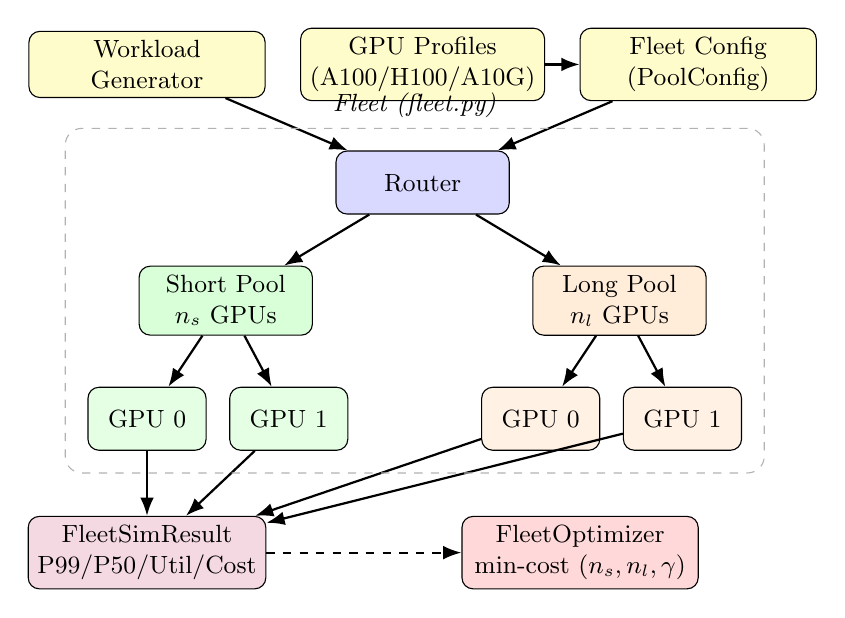
\begin{tikzpicture}[
  box/.style={rectangle, rounded corners=4pt, draw, minimum width=3cm,
    minimum height=0.8cm, align=center, font=\small},
  arrow/.style={-Latex, thick},
  group/.style={rectangle, rounded corners=6pt, draw=gray!60,
    dashed, inner sep=8pt},
]
% Inputs
\node[box, fill=yellow!20] (wl) at (0, 4) {Workload\\Generator};
\node[box, fill=yellow!20] (gpu) at (3.5, 4) {GPU Profiles\\(A100/H100/A10G)};
\node[box, fill=yellow!20] (cfg) at (7, 4) {Fleet Config\\(PoolConfig)};

% Fleet
\node[box, fill=blue!15, minimum width=2.2cm] (router) at (3.5, 2.5) {Router};
\node[box, fill=green!15, minimum width=2.2cm] (sp) at (1, 1) {Short Pool\\$n_s$ GPUs};
\node[box, fill=orange!15, minimum width=2.2cm] (lp) at (6, 1) {Long Pool\\$n_l$ GPUs};
\node[box, fill=green!10, minimum width=1.5cm] (i1) at (0, -0.5) {GPU 0};
\node[box, fill=green!10, minimum width=1.5cm] (i2) at (1.8, -0.5) {GPU 1};
\node[box, fill=orange!10, minimum width=1.5cm] (j1) at (5, -0.5) {GPU 0};
\node[box, fill=orange!10, minimum width=1.5cm] (j2) at (6.8, -0.5) {GPU 1};

% Outputs
\node[box, fill=purple!15] (res) at (0, -2.2) {FleetSimResult\\P99/P50/Util/Cost};
\node[box, fill=red!15] (opt) at (5.5, -2.2) {FleetOptimizer\\min-cost $(n_s,n_l,\gamma)$};

% Arrows
\draw[arrow] (wl) -- (router);
\draw[arrow] (gpu) -- (cfg);
\draw[arrow] (cfg) -- (router);
\draw[arrow] (router) -- (sp);
\draw[arrow] (router) -- (lp);
\draw[arrow] (sp) -- (i1); \draw[arrow] (sp) -- (i2);
\draw[arrow] (lp) -- (j1); \draw[arrow] (lp) -- (j2);
\draw[arrow] (i1) -- (res); \draw[arrow] (i2) -- (res);
\draw[arrow] (j1) -- (res); \draw[arrow] (j2) -- (res);
\draw[arrow, dashed] (res) -- (opt);

\node[group, fit=(router)(sp)(lp)(i1)(i2)(j1)(j2),
  label=above:{\small\textit{Fleet (fleet.py)}}] {};
\end{tikzpicture}
\caption{High-level component diagram.  Each GPU instance runs an
  M/G/$c$-style discrete-event simulation.}
\label{fig:architecture}
\end{figure}

The simulator has four layers:

\begin{enumerate}[nosep]
  \item \textbf{Workload} (\texttt{fleet\_sim/workload/}) --- generates
    request arrivals with a Poisson process.  Supports empirical CDFs
    (from JSON files) and synthetic Poisson distributions.

  \item \textbf{GPU Profiles} (\texttt{fleet\_sim/gpu\_profiles/}) ---
    hardware constants $(W, H, n_{\max}, C_{\max})$ for each GPU type.
    Pre-defined: A100-80GB, H100-80GB, A10G.

  \item \textbf{Core} (\texttt{fleet\_sim/core/}) --- the simulation
    engine:
    \begin{itemize}[nosep]
      \item \texttt{request.py}: \texttt{Request} dataclass, lifecycle
        states (\textsc{Waiting} $\to$ \textsc{Prefill} $\to$
        \textsc{Decoding} $\to$ \textsc{Done}).
      \item \texttt{instance.py}: single GPU; implements fast
        request-level DES using a min-heap event queue.  Each request
        triggers exactly two events: arrival and completion.
      \item \texttt{pool.py}: $c$ GPU instances behind a shared queue;
        load balancing across instances.
      \item \texttt{fleet.py}: two pools + router; drives the
        simulation clock, collects \texttt{FleetSimResult}.
    \end{itemize}

  \item \textbf{Routing} (\texttt{fleet\_sim/routing/}) --- pluggable
    routing algorithms (Section~\ref{sec:routing}).

  \item \textbf{Optimizer} (\texttt{fleet\_sim/optimizer.py}) --- two-phase
    analytical sweep + DES verification to find minimum-cost fleet.
\end{enumerate}

\subsection{Request Lifecycle}

A request passes through these stages:

\begin{center}
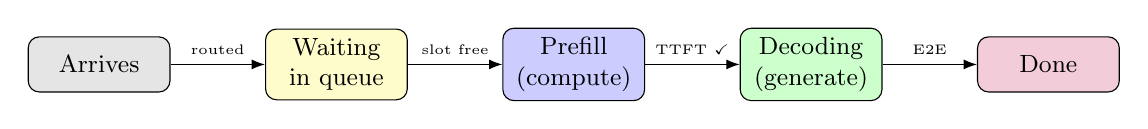
\begin{tikzpicture}[
  state/.style={rectangle, rounded corners, draw, minimum width=1.8cm,
    minimum height=0.7cm, align=center, font=\small},
  arrow/.style={-Latex},
]
\node[state, fill=gray!20] (arr) {Arrives};
\node[state, fill=yellow!20, right=1.2cm of arr] (wait) {Waiting\\in queue};
\node[state, fill=blue!20, right=1.2cm of wait] (pre) {Prefill\\(compute)};
\node[state, fill=green!20, right=1.2cm of pre] (dec) {Decoding\\(generate)};
\node[state, fill=purple!20, right=1.2cm of dec] (done) {Done};
\draw[arrow] (arr) -- node[above,font=\tiny]{routed} (wait);
\draw[arrow] (wait) -- node[above,font=\tiny]{slot free} (pre);
\draw[arrow] (pre) -- node[above,font=\tiny]{TTFT \checkmark} (dec);
\draw[arrow] (dec) -- node[above,font=\tiny]{E2E} (done);
\end{tikzpicture}
\end{center}

Measured metrics per request:
\begin{itemize}[nosep]
  \item \textbf{queue\_wait}: time from arrival until a GPU slot is
    assigned
  \item \textbf{ttft}: time from arrival to first output token
    (= queue\_wait + prefill + 1 decode step)
  \item \textbf{e2e\_latency}: time from arrival to last token
\end{itemize}

\subsection{Fast Instance Simulation}

Each GPU instance uses a \textbf{request-level event model} rather
than token-by-token simulation.  For a request with $L_{\text{in}}$
input and $L_{\text{out}}$ output tokens, the simulator computes
upfront:
\begin{align}
  S_{\text{raw}} &= (\text{prefill\_iters} + L_{\text{out}}) \times t_{\text{iter}},\\
  S_{\text{eff}} &= S_{\text{raw}} / n_{\max}.  \quad \text{(slot freed for scheduling)}
\end{align}
Two events are inserted into a min-heap: a TTFT event at
\texttt{now + prefill\_iters * iter\_t}, and a completion event at
\texttt{now + S\_eff}.  This is $O(\log n)$ per request rather than
$O(L_{\text{out}})$, enabling simulation of millions of requests per
second.

\subsection{Available Routing Algorithms}
\label{sec:routing}

\begin{center}
\begin{tabular}{lp{9cm}}
\toprule
Router & Behaviour \\
\midrule
\texttt{LengthRouter} & Routes to the smallest pool whose \texttt{max\_ctx}
  fits the request.  Default for length-partitioned fleets. \\
\texttt{CompressAndRouteRouter} & Like \texttt{LengthRouter} but compresses
  borderline requests in $(\Bshort, \gamma\Bshort]$ to the short pool. \\
\texttt{ModelRouter} & Routes each request to the pool matching
  \texttt{request.model\_id}; falls back to the default pool. \\
\texttt{SemanticRouter} & Routes using a user-supplied
  \texttt{classify\_fn(Request) $\to$ pool\_id}.  Supports any
  classifier: intent detection, embedding lookup, keyword rules, LLM
  judge.  See Section~\ref{sec:semantic}. \\
\texttt{LeastLoadedRouter} & Sends each request to the pool with the
  fewest queued requests (runtime state). \\
\texttt{RandomRouter} & Uniform random assignment.  Baseline. \\
\bottomrule
\end{tabular}
\end{center}

\begin{keyinsight}
  Pool routing by prompt length is \textbf{one use case} of the
  simulator.  A fleet may have $N$ pools distinguished by model,
  hardware tier, or any other criterion.  Use \texttt{ModelRouter},
  \texttt{SemanticRouter}, or the \texttt{simulate-fleet} CLI command
  (Section~\ref{sec:multipool}) for these topologies.
\end{keyinsight}

% ====================================================================
\section{Quick Start}
\label{sec:quickstart}

\subsection{Installation}

\begin{lstlisting}[style=shell]
git clone https://github.com/vllm-project/semantic-router
cd semantic-router/bench/fleet-simulator
pip install -r requirements.txt    # numpy, scipy only
\end{lstlisting}

The simulator has no GPU or ML framework dependencies --- it runs
entirely in CPU-only Python.

\subsection{Your First Run: Size a Fleet in 30 Seconds}

\begin{lstlisting}[style=shell]
python run_sim.py optimize \
  --cdf data/azure_cdf.json \
  --lam 200 --slo 500 --b-short 6144 \
  --gpu-short a100 --gpu-long a100
\end{lstlisting}

This finds the minimum-cost A100 fleet for 200 req/s Azure traffic
at P99 TTFT $\leq$ 500\,ms with a 6K-token pool boundary.
It takes about 2\,seconds.  The output is shown in
Section~\ref{sec:cs-optimize}.

\subsection{Data Format}

The \texttt{--cdf} argument expects a JSON file with a list of
\texttt{[token\_length, cumulative\_fraction]} pairs:

\begin{lstlisting}[style=python]
# azure_cdf.json (excerpt)
[
  [128,  0.028],
  [256,  0.068],
  [512,  0.289],
  [1024, 0.404],
  [2048, 0.780],
  [4096, 0.898],
  [6144, 0.976],
  [8192, 1.000],
  ...
]
\end{lstlisting}

The simulator interpolates linearly between points.  You can generate
a CDF from any request log using the helper in
\texttt{fleet\_sim/workload/trace.py}.

\subsection{Available GPU Profiles}

\begin{center}
\begin{tabular}{lrrrrl}
\toprule
Profile & $W$ (ms) & $H$ (ms/slot) & $n_{\max}$ (short) & $n_{\max}$ (long)
  & Typical use \\
\midrule
\texttt{a100} & 8.0 & 0.65 & 128 & 16 & General purpose \\
\texttt{h100} & 4.0 & 0.32 & 128 & 16 & Low-latency SLO \\
\texttt{a10g} & 12.0 & 0.90 & 64  & 8  & Cost-sensitive long pool \\
\bottomrule
\end{tabular}
\end{center}

Pre-built profiles are calibrated for Llama-3-70B.
Use \texttt{CUSTOM(name, W, H, ...)} to supply your own constants,
or \texttt{ProfileBuilder} to compute them from hardware and model specs.

\subsection{Physics-Informed Profiles via \texttt{ProfileBuilder}}
\label{sec:computed-profiles}

The simulator can derive $W$, $H$, and \texttt{total\_kv\_blks}
from first principles using a \emph{hardware spec} $\times$ \emph{model spec}
pair, inspired by the bottom-up roofline approach of
AIConfigurator~\citep{xu2025aiconfigurator}.

\paragraph{Hardware catalog.}
Eight pre-built \texttt{HardwareSpec} instances cover all current NVIDIA
generations (A100, L40S, B60, H100 SXM, H200 SXM, B200 SXM, GB200 NVL,
GB300 NVL).  Each spec records peak memory bandwidth, VRAM capacity, FP16/FP8
TC TFLOPS, TDP, and estimated cloud cost.  Empirical constants from
AIConfigurator's silicon measurements are embedded directly:

\begin{center}
\begin{tabular}{ll}
\toprule
Constant & Value \\
\midrule
Memory bandwidth scale factor & 0.80 (achievable fraction of peak) \\
Per-layer constant latency & 3\,\textmu s (NCCL + kernel launch) \\
NCCL overhead, TP=2 & 0.5\,GB reserved \\
NCCL overhead, TP=4 & 1.0\,GB reserved \\
NCCL overhead, TP=8 & 2.0\,GB reserved \\
\bottomrule
\end{tabular}
\end{center}

\paragraph{Model catalog.}
Ten \texttt{ModelSpec} instances cover Llama-3.1 (8B, 70B, 405B),
Qwen3 (8B, 32B, 30B-A3B, 235B-A22B), and DeepSeek-V3.
Each spec includes layer count, hidden dimension, GQA KV-head count,
and MoE configuration (number of experts, top-$k$ routing).

\paragraph{Dense model formulas.}
For a dense model with $P$ parameters split across $T_P$ tensor-parallel
GPUs, loaded in $d$ bytes per weight, the iteration latency parameters are:

\[
  W \;=\; \frac{P \cdot d / T_P}{B_{\text{mem}} \cdot 0.80} \;+\;
          L \cdot 3\,\mu\text{s}
\]
\[
  H \;=\; \frac{k_{\text{KV/token}} / T_P}{B_{\text{mem}} \cdot 0.80}
          \;\cdot\; \bar{C}
\]

where $B_{\text{mem}}$ is peak GPU memory bandwidth, $L$ is the number of
layers, $k_{\text{KV/token}}$ is the KV-cache bytes per sequence token (all
layers), and $\bar{C}$ is the representative context length (set via
\texttt{ServingConfig.mean\_ctx\_tokens}).

\paragraph{MoE models.}
MoE models use a silicon-measured kernel lookup table (\texttt{\_MOE\_TABLE}
in \texttt{builder.py}) containing H100 SXM latencies for DeepSeek-V3 and
Qwen3 variants across FP16/FP8/INT4 quantization.  Results are
interpolated for intermediate token counts and scaled to other GPUs by
memory-bandwidth ratio.

\paragraph{Example usage.}

\begin{lstlisting}[style=python]
from fleet_sim import H100_SXM, LLAMA_3_1_70B
from fleet_sim.gpu_profiles import ProfileBuilder, ServingConfig

profile = ProfileBuilder().build(
    H100_SXM,
    LLAMA_3_1_70B,
    ServingConfig(tp=8, dtype_bytes=2, mean_ctx_tokens=2048),
)
print(profile.summary())
# H100-SXM | Llama-3.1-70B | TP8 FP16
#   W = 5.82 ms   H = 0.039 ms/seq   KV blocks = 4271  cost = $32.16/hr
\end{lstlisting}

The resulting \texttt{ComputedProfile} satisfies the \texttt{GpuProfile}
Protocol and can be used anywhere a \texttt{ManualProfile} would be
used --- in \texttt{PoolConfig}, the \texttt{FleetOptimizer}, or the
\texttt{DisaggFleetOptimizer}.

\subsection{Disaggregated Fleet Optimizer}
\label{sec:disagg-optimizer}

\texttt{DisaggFleetOptimizer} sizes separate prefill and decode worker pools
following the rate-matching approach of
AIConfigurator~\citep{xu2025aiconfigurator}.  Each pool runs with its own
tensor-parallelism degree and quantization setting.

Two empirical degradation factors account for the overhead of
KV-transfer between prefill and decode nodes in a disaggregated deployment:

\[
  R_{\text{sys}} = \min\!\bigl(
    n_{\text{pre}} \cdot \mu_{\text{pre}} \cdot \alpha_{\text{pre}},\;
    n_{\text{dec}} \cdot \mu_{\text{dec}} \cdot \alpha_{\text{dec}}
  \bigr)
\]
\[
  \text{TTFT}_{\text{eff}} = T_{\text{prefill}} \cdot \beta_{\text{TTFT}}
\]

\noindent
with embedded constants $\alpha_{\text{pre}} = 0.90$,
$\alpha_{\text{dec}} = 0.92$, $\beta_{\text{TTFT}} = 1.80$
(measured in~\citealt{xu2025aiconfigurator}).

\begin{lstlisting}[style=python]
from fleet_sim import DisaggFleetOptimizer, H100_SXM, LLAMA_3_1_70B
from fleet_sim.gpu_profiles import ProfileBuilder, ServingConfig

builder = ProfileBuilder()
prefill = builder.build(H100_SXM, LLAMA_3_1_70B,
    ServingConfig(tp=4, dtype_bytes=2, mean_ctx_tokens=1024, phase="prefill"))
decode  = builder.build(H100_SXM, LLAMA_3_1_70B,
    ServingConfig(tp=8, dtype_bytes=2, mean_ctx_tokens=1024, phase="decode"))

opt = DisaggFleetOptimizer(
    prefill_profile=prefill, decode_profile=decode,
    mean_isl=1024, mean_osl=256,
    slo_ttft_ms=2000, slo_tpot_ms=100, max_ctx=4096,
)
result = opt.optimize(max_prefill=8, max_decode=8)
result.print_report()
# Disaggregated fleet:  4x prefill (TP4)  +  6x decode (TP8)
#   System rate: 87.3 req/s   TTFT: 1842 ms   TPOT: 94.1 ms
#   Total GPUs: 64   Cost: $257.2/hr
\end{lstlisting}

% ====================================================================
\section{CLI Reference}
\label{sec:cli}

\subsection{\texttt{optimize}: Find the Minimum-Cost Fleet}

\begin{lstlisting}[style=shell]
python run_sim.py optimize \
  --cdf PATH           # workload CDF JSON (required)
  --lam FLOAT          # arrival rate (req/s, default: 100)
  --slo FLOAT          # P99 TTFT budget (ms, default: 500)
  --b-short INT        # pool boundary tokens (default: 8192)
  --long-max-ctx INT   # long-pool max context (default: 65536)
  --gpu-short TYPE     # a100 | h100 | a10g (default: a100)
  --gpu-long  TYPE     # a100 | h100 | a10g (default: a100)
  --gamma-max FLOAT    # max C&R bandwidth to sweep (default: 2.0)
  --verify-top INT     # DES-verify top-N analytical candidates (3)
  --out PATH           # save JSON results to file
\end{lstlisting}

\textbf{Algorithm}: two-phase search.
Phase 1 sweeps $\gamma \in \{1.0, 1.1, \ldots, \gamma_{\max}\}$ using
the analytical M/G/$c$ model to score each configuration.
Phase 2 runs DES on the top-\texttt{verify-top} candidates and
returns the best DES-verified result.

\subsection{\texttt{simulate}: Evaluate a Fixed Fleet}

\begin{lstlisting}[style=shell]
python run_sim.py simulate \
  --cdf PATH --lam FLOAT --slo FLOAT \
  --b-short INT --gpu-short TYPE --gpu-long TYPE \
  --n-s INT            # short-pool GPU count (required)
  --n-l INT            # long-pool GPU count (required)
  --gamma FLOAT        # C&R gamma (1.0 = no compression, default)
  --n-req INT          # requests to simulate (default: 10000)
  --seed INT           # random seed (default: 42)
  --out PATH
\end{lstlisting}

Use this to \textbf{validate} a fleet you already have, or to test a
specific configuration the optimizer didn't propose.

\subsection{\texttt{whatif}: Traffic Spike and Growth Analysis}

\begin{lstlisting}[style=shell]
python run_sim.py whatif \
  --cdf PATH --slo FLOAT --b-short INT \
  --gpu-short TYPE --gpu-long TYPE \
  --lam-range 50 100 150 200 250 300   # list of rates to sweep
  --out PATH
\end{lstlisting}

Runs \texttt{optimize} at each $\lambda$ in the range and prints a
table of optimal fleet sizes and costs.  Essential for capacity
planning over a multi-quarter growth forecast.

\subsection{\texttt{compare-routers}: Router Benchmarking}

\begin{lstlisting}[style=shell]
python run_sim.py compare-routers \
  --cdf PATH --lam FLOAT --slo FLOAT \
  --b-short INT --gpu-short TYPE --gpu-long TYPE \
  --n-s INT --n-l INT  # fixed fleet size for all routers
  --n-req INT --seed INT
\end{lstlisting}

Runs the same fixed fleet under all available routing algorithms
and compares P99 TTFT, SLO compliance, and utilization.

\subsection{\texttt{grid-flex}: Power–Latency Trade-off for Demand Response}
\label{sec:cli-grid-flex}

\begin{lstlisting}[style=shell]
python run_sim.py grid-flex \
  --cdf PATH           # workload CDF JSON (required)
  --lam FLOAT          # arrival rate (req/s)
  --n-gpus INT         # fixed fleet size to evaluate (required)
  --gpu TYPE           # a100 | h100 | a10g (default: h100)
  --slo FLOAT          # P99 TTFT SLO (ms, default: 500)
  --max-ctx INT        # max context window (tokens, default: 8192)
  --flex-pcts F1 F2... # power-reduction percentages to sweep
                       # (default: 0 5 10 15 20 25 30 40 50)
  --out PATH           # save results to JSON
\end{lstlisting}

\textbf{What it does.}
Sweeps power-reduction target percentages and, for each one, reports:
(1) the implied batch-size cap $n_{\max}$ derived by inverting the GPU power
model; (2) estimated per-GPU power draw (W) and total fleet power (kW);
(3) analytical P99 TTFT at the reduced concurrency; and (4) whether the
SLO is still met.  The table closes with the \emph{maximum safe flex depth}
--- the largest curtailment that still meets the SLO.

\textbf{Use case.}
Operators enrolled in utility demand-response (DR) programmes must commit
to a power reduction level in advance.  This command answers: \emph{``how
much power can I offer without breaching my latency SLA?''}

\textbf{Power model.}
Each GPU profile stores \texttt{power\_idle\_w} (power at batch~$\approx 1$)
and \texttt{power\_nominal\_w} (power at full \texttt{max\_slots} concurrency),
sourced from ML.ENERGY Benchmark v3.0 measurements on H100-SXM5
and NVIDIA spec sheets.  Power is linearly interpolated between these two
scalars --- a conservative approximation accurate to within $\pm 5\%$ in the
40--100\% load range relevant for DR operations.

\textbf{Example output} (30 H100s, $\lambda = 300$\,req/s, SLO\,=\,200\,ms):

\begin{lstlisting}[style=output]
======================================================================
  Grid Flexibility Analysis
  Fleet: 30 GPUs  lam=300 req/s  SLO=200 ms
  Baseline: 13.5 kW fleet power  (450 W/GPU)
======================================================================
  Flex  n_max   W/GPU  Fleet kW  P99 TTFT   SLO
------  -----  ------  --------  --------   ---
    0%    128   450W    13.5kW      7.9ms    OK
    5%    115   435W    13.0kW      7.9ms    OK
   10%    102   420W    12.6kW      7.9ms    OK
   15%     90   405W    12.2kW      7.9ms    OK
   20%     77   390W    11.7kW      7.9ms    OK
   25%     64   375W    11.2kW   1058.2ms  BREACH
   30%     51   360W    10.8kW    inf ms   BREACH
   40%     26   330W     9.9kW    inf ms   BREACH

  Max safe flex depth: 20%  (saves 1.8 kW, P99=7.9ms)
\end{lstlisting}

The abrupt transition at 25\% corresponds to the Erlang-C saturation
threshold: below $n_{\max} = 64$ the arrival load exceeds the available
KV-slot count and the queue diverges.  The simulator locates this cliff
analytically, before any hardware change.

% ====================================================================
\section{Case Studies}
\label{sec:casestudies}

\subsection{Case Study 1: ``How Many GPUs Do I Need?''}
\label{sec:cs-optimize}

\textbf{Scenario.}  You are launching an LLM API backed by Llama-3-70B
on A100-80GB GPUs.  Historical traffic analysis gives you the Azure
conversational CDF.  You expect 200 requests/second at peak and
need P99 TTFT $\leq$ 500\,ms.  The pool boundary is set at 6,144 tokens
(the CDF knee, where $F(\Bshort) \approx 0.976$).

\textbf{Command.}
\begin{lstlisting}[style=shell]
python run_sim.py optimize \
  --cdf data/azure_cdf.json \
  --lam 200 --slo 500 --b-short 6144 \
  --gpu-short a100 --gpu-long a100
\end{lstlisting}

\textbf{Output.}
\begin{lstlisting}[style=output]
[1/2] Analytical sweep over gamma in [1.0 .. 2.0] ...
[2/2] DES verification of top-3 candidates...
  Verifying gamma=1.3 (n_s=50, n_l=10)...
    P99 short=80.9ms  long=392.0ms  SLO:PASS
  Verifying gamma=1.2 (n_s=50, n_l=11)...
    P99 short=78.6ms  long=411.8ms  SLO:PASS
  Verifying gamma=1.0 (n_s=49, n_l=13)...
    P99 short=91.2ms  long=450.0ms  SLO:PASS

Fleet Optimization Report
B_short=6,144  lambda=200 req/s  SLO=500ms

Best (analytical): gamma=1.3  n_s=50  n_l=10  total=60  $1161.6K/yr
Best (simulated):  gamma=1.3  n_s=50  n_l=10  total=60  $1161.6K/yr
  P99 TTFT: short=80.9ms  long=392.0ms  SLO:PASS

gamma sweep (analytical, baseline=gamma=1.0 with 62 GPUs):
  gamma  n_s  n_l  total    $K/yr  saving   P99_s    P99_l
    1.0   49   13     62  $1200K   +0.0%   75.9ms  356.2ms
    1.1   50   12     62  $1200K   -0.0%   62.9ms  368.5ms
    1.2   50   11     61  $1181K   +1.6%   65.1ms  348.1ms
    1.3   50   10     60  $1162K   +3.2%   67.4ms  295.0ms  <-- best
    1.4   50   14     64  $1239K   -3.2%   68.2ms  471.6ms
    ...
\end{lstlisting}

\textbf{Interpretation.}
\begin{itemize}[nosep]
  \item You need \textbf{60 GPUs} (50 short, 10 long).  A homogeneous
    fleet where all GPUs handle full 64K context would require $\sim$90
    GPUs (see Case Study~4).
  \item Setting $\gamma = 1.3$ (compress borderline requests up to
    30\% over the boundary) saves 2 GPUs (\$38K/yr) vs.\ plain pool
    routing at $\gamma = 1.0$.
  \item Both pools pass the 500\,ms SLO comfortably: 81\,ms and
    392\,ms respectively.
  \item The DES result matches the analytical prediction exactly
    (same fleet chosen), confirming the model is not overly optimistic.
\end{itemize}

\begin{keyinsight}
  The analytical sweep is the right starting point.
  DES verification is a safety check: if the analytical and DES
  choices agree, you can trust the analytical model for faster
  iteration.  If they disagree, always trust the DES result.
\end{keyinsight}

\subsection{Case Study 2: ``Will My Fleet Survive Traffic Growth?''}
\label{sec:cs-whatif}

\textbf{Scenario.}  Your fleet runs at 200\,req/s today but your
growth model forecasts 300\,req/s in Q3.  You want to know the
GPU count and annual cost at each point so you can plan procurement.

\textbf{Command.}
\begin{lstlisting}[style=shell]
python run_sim.py whatif \
  --cdf data/azure_cdf.json \
  --slo 500 --b-short 6144 \
  --gpu-short a100 --gpu-long a100 \
  --lam-range 50 100 150 200 250 300
\end{lstlisting}

\textbf{Output.}
\begin{lstlisting}[style=output]
What-if analysis: sweep lambda over [50, 100, 150, 200, 250, 300]
B_short=6,144  SLO=500.0ms  GPU: A100-80GB/A100-80GB

  lambda  n_s  n_l  total    $K/yr   gamma*   P99_s    P99_l
  ---------------------------------------------------------
      50   13    5     18  $ 348.5K    1.1  266.9ms  384.5ms
     100   25    6     31  $ 600.1K    1.3  165.0ms  477.4ms
     150   37    9     46  $ 890.5K    1.2  110.0ms  364.6ms
     200   50   10     60  $1161.6K   1.3   67.4ms  295.0ms
     250   62   11     73  $1413.3K   1.3   53.8ms  432.1ms
     300   74   14     88  $1703.6K   1.2   42.0ms  476.4ms
\end{lstlisting}

\textbf{Interpretation.}
\begin{itemize}[nosep]
  \item GPU count scales sub-linearly with $\lambda$: from 18 GPUs
    at 50\,req/s to 88 GPUs at 300\,req/s (4.9$\times$ the GPUs
    for 6$\times$ the traffic).  This is the Erlang-C ``economy of
    scale'' effect: larger fleets run at lower per-GPU utilization
    for the same SLO.
  \item Annual cost grows from \$349K to \$1.7M as traffic scales
    6$\times$.  You can share this table directly with finance for
    infrastructure budget planning.
  \item The optimal $\gamma^*$ fluctuates (1.1--1.3) because the
    Erlang-C discrete GPU counts create a staircase: at each $\lambda$,
    a slightly different $\gamma$ minimizes the integer-rounded GPU count.
  \item The long pool consistently stays near the SLO limit (384--477\,ms),
    while the short pool has plenty of headroom.  If the SLO tightens
    to 300\,ms, the long-pool sizing would become the bottleneck first.
\end{itemize}

\begin{keyinsight}
  The \texttt{whatif} output is a procurement plan.  Use
  \texttt{--out growth\_plan.json} to save the full results and feed
  them into your infrastructure cost model.
\end{keyinsight}

\subsection{Case Study 3: ``Which Router Should I Use for Agent Traffic?''}
\label{sec:cs-routers}

\textbf{Scenario.}  Your workload is shifting toward agent-heavy
traffic (long RAG contexts, tool calls).  You have a fixed fleet
of 60 short + 50 long GPUs at $\lambda = 100$\,req/s and want to
know whether switching from \texttt{LengthRouter} to
\texttt{CompressAndRouteRouter} or \texttt{LeastLoadedRouter}
improves P99 TTFT.

\textbf{Command.}
\begin{lstlisting}[style=shell]
python run_sim.py compare-routers \
  --cdf data/agent_heavy_cdf.json \
  --lam 100 --slo 500 --b-short 16384 \
  --n-s 60 --n-l 50 \
  --gpu-short a100 --gpu-long a100
\end{lstlisting}

\textbf{Output.}
\begin{lstlisting}[style=output]
Router comparison  lambda=100 req/s  n_s=60 n_l=50  SLO=500.0ms
Router                         P99 TTFT     SLO%     Util
----------------------------------------------------------
LengthRouter                   1328.2ms   66.42%     2.5%
CompressAndRouteRouter         1306.4ms   66.16%     2.2%
RandomRouter                   2182.4ms   78.15%     3.1%
\end{lstlisting}

\textbf{Interpretation.}
\begin{itemize}[nosep]
  \item All three routers fail the 500\,ms SLO at this fleet size
    for agent-heavy traffic.  The issue is \emph{not} the router
    choice --- it is fleet under-provisioning.  With only 110 GPUs
    at 100\,req/s for this workload, utilization is low (2.5\%) but
    P99 TTFT is 1.3\,s.  The bottleneck is \textbf{prefill time for
    long requests}, not queueing: agent-heavy requests with
    $L_{\text{in}} = 20{,}000$ tokens take
    $\lceil 20{,}000/512 \rceil \times 8\,\text{ms} \approx 312\,\text{ms}$
    of prefill alone.
  \item \texttt{CompressAndRouteRouter} gives a small improvement
    (1.6\% reduction in P99 TTFT) by redirecting borderline requests
    to the faster short pool.
  \item \texttt{RandomRouter} is significantly worse: it ignores
    token lengths and sends long requests to the short pool, causing
    KV-cache pressure and long queueing.
  \item \textbf{Action}: run \texttt{optimize} first to get the right
    fleet size, then use \texttt{compare-routers} to fine-tune the
    routing algorithm on the correctly-sized fleet.
\end{itemize}

\begin{warning}
  A low utilization reading ($< 5\%$) does not mean the fleet is
  over-provisioned.  For long-context workloads, P99 TTFT is dominated
  by \textbf{prefill time}, which is fixed by $L_{\text{in}}$ and
  independent of utilization.  You cannot reduce prefill time by
  adding GPUs; you can reduce it by lowering $\Bshort$ or using C\&R.
\end{warning}

\subsection{Case Study 4: ``Homogeneous vs.\ Two-Pool: Is It Worth the Complexity?''}
\label{sec:cs-savings}

\textbf{Scenario.}  Your team is debating whether to operate two
separate GPU pools (short + long) versus one homogeneous fleet.
The two-pool setup requires a router and separate queues.  You want
to quantify the cost savings to justify the operational complexity.

\textbf{Approach.}  Run \texttt{optimize} on the homogeneous
architecture first (by setting \texttt{--b-short 1} so all traffic
routes to the long pool, which is configured for 64K context),
then compare with the two-pool result.

\textbf{Step 1: Find the minimum homogeneous fleet.}
\begin{lstlisting}[style=shell]
# All traffic goes to long pool (64K context, 16 slots/GPU)
python run_sim.py optimize \
  --cdf data/azure_cdf.json \
  --lam 200 --slo 500 --b-short 1 \
  --long-max-ctx 65536 \
  --gpu-short a100 --gpu-long a100
# Result: n_l=88 GPUs  $1,742K/yr  P99 queue wait=113.6ms
\end{lstlisting}

\textbf{Step 2: Two-pool fleet} (from Case Study~1):
\begin{lstlisting}[style=shell]
python run_sim.py optimize \
  --cdf data/azure_cdf.json \
  --lam 200 --slo 500 --b-short 6144 \
  --gpu-short a100 --gpu-long a100
# Result: n_s=50 n_l=10  total=60  $1,162K/yr
\end{lstlisting}

\textbf{Results summary.}
\begin{center}
\begin{tabular}{lrrrl}
\toprule
Architecture & GPUs & Ann.\ cost & P99 queue wait & SLO \\
\midrule
Homogeneous (64K context)  & 90 & \$1.74M & 114\,ms & \checkmark \\
Two-pool (\texttt{b-short}=6K) & 60 & \$1.16M & 81\,ms & \checkmark \\
\midrule
\textbf{Saving} & \textbf{30 GPUs} & \textbf{\$581K/yr (33\%)} & --- & --- \\
\bottomrule
\end{tabular}
\end{center}

\textbf{Interpretation.}  The two-pool architecture saves
\textbf{33\% of GPU cost} (\$581K/yr at \$2.21/GPU-hr) by routing
the $\sim$97.6\% of requests below 6K tokens to the efficient
short pool ($8\times$ throughput per GPU vs.\ long pool).

\begin{warning}
  The table reports \emph{P99 queue wait}, which is what the
  analytical model and the optimizer's fast DES measure.  If you
  run \texttt{simulate} with the two-pool fleet, the \emph{full}
  P99 TTFT will be $\sim$912\,ms --- exceeding the 500\,ms SLO ---
  because for $\Bshort = 6{,}144$-token requests, prefill time
  alone is $\lceil 4{,}915/512 \rceil \times 91.2\,\text{ms}
  \approx 912\,\text{ms}$.  This is the prefill-dominated regime
  described in Section~\ref{sec:ttft}: the SLO budget is consumed
  by compute, not queueing.  To fit a 500\,ms wall-clock SLO, set
  $\Bshort \leq 2{,}048$ or account for prefill time when
  interpreting the optimizer's output.
\end{warning}

The operational complexity of a second pool and a router is
amortised in under two weeks of GPU cost savings at this scale.

\subsection{Case Study 5: ``Semantic Router --- Sizing a Two-Model Fleet''}
\label{sec:cs-semantic}

\textbf{Scenario.}  You are deploying a semantic router that classifies
incoming Azure-like traffic (200\,req/s, 500\,ms P99 TTFT SLO) into two
streams:

\begin{itemize}[nosep]
  \item \textbf{Simple queries} (70\% of traffic, 140\,req/s) routed to a
    cost-efficient \texttt{llama8b} model on A10G GPUs (max context~4K).
  \item \textbf{Complex queries} (30\% of traffic, 60\,req/s) routed to a
    high-capability \texttt{llama70b} model on A100-80GB GPUs (max context~8K).
\end{itemize}

You want to determine the right GPU count for each pool and quantify the
cost savings versus a homogeneous A100 fleet that serves all traffic with
the large model.

\textbf{Step 1: Optimize the small-model pool (A10G, 140\,req/s).}

\begin{lstlisting}[style=shell]
# All traffic routed to single short pool (b_short=65536 >> any request)
python run_sim.py optimize \
  --cdf data/azure_cdf.json --lam 140 --slo 500 \
  --b-short 65536 --gpu-short a10g --gpu-long a10g
# Best (simulated): n_s=129 n_l=0  total=129  $1,141K/yr
#   P99 TTFT: short=114.7ms  SLO: pass
\end{lstlisting}

\textbf{Step 2: Optimize the large-model pool (A100, 60\,req/s).}

\begin{lstlisting}[style=shell]
python run_sim.py optimize \
  --cdf data/lmsys_cdf.json --lam 60 --slo 500 \
  --b-short 65536 --long-max-ctx 8192 \
  --gpu-short a100 --gpu-long a100
# Best (simulated): n_s=13  n_l=0  total=13  $252K/yr
#   P99 TTFT: short=253.8ms  SLO: pass
\end{lstlisting}

\textbf{Step 3: Homogeneous A100 baseline (no semantic routing).}

\begin{lstlisting}[style=shell]
python run_sim.py optimize \
  --cdf data/azure_cdf.json --lam 200 --slo 500 \
  --b-short 65536 --gpu-short a100 --gpu-long a100
# Best (simulated): n_s=88  n_l=0  total=88  $1,704K/yr
#   P99 TTFT: short=84.7ms  SLO: pass
\end{lstlisting}

\textbf{Results.}
\begin{center}
\begin{tabular}{lrrrl}
\toprule
Configuration & GPUs & Ann.\ cost & P99 TTFT & SLO \\
\midrule
Homogeneous A100 (large model only) & 88 A100 & \$1.70M & 84.7\,ms & \checkmark \\
Semantic: \texttt{llama8b} pool (A10G) & 129 A10G & \$1.14M & 114.7\,ms & \checkmark \\
Semantic: \texttt{llama70b} pool (A100) & 13 A100 & \$0.25M & 253.8\,ms & \checkmark \\
\midrule
\textbf{Semantic fleet total} & 142 & \textbf{\$1.39M} & --- & \checkmark \\
\textbf{Saving vs.\ homogeneous} & +54 GPUs & \textbf{\$311K/yr (18\%)} & --- & --- \\
\bottomrule
\end{tabular}
\end{center}

\textbf{Interpretation.}  Despite requiring 54 \emph{more} GPUs in total,
the semantic fleet costs 18\% less because A10G GPUs (\$1.01/GPU-hr) are
less than half the price of A100s (\$2.21/GPU-hr), and 70\% of traffic can
be served by the cheaper hardware.  The large-model pool (13 A100s) handles
only the 30\% of complex traffic, keeping utilisation comfortable.

\begin{keyinsight}
  In the semantic-routing scenario the cost saving comes from
  \textbf{hardware heterogeneity}, not from increased GPU utilisation.
  Use the \texttt{--gpu-short} / \texttt{--gpu-long} flags in each
  \texttt{optimize} call to model your actual GPU mix.  Then replay a
  production access log (Section~\ref{sec:semantic-full}) to validate
  that the routing distribution matches the CDF assumption.
\end{keyinsight}

% ====================================================================
\subsection{Case Study 6: ``How Much Power Can I Offer the Grid?''}
\label{sec:cs-grid-flex}

\textbf{Scenario.}
Your data center participates in a utility demand-response (DR) programme.
On short notice (15--60 minutes), the grid operator can request a power
reduction of up to 30\%.  You run 30 H100-80GB GPUs serving an Azure-like
workload at $\lambda = 300$\,req/s with a P99 TTFT SLO of 200\,ms.  You
need to know: how deep a curtailment commitment can you sign up for without
risking an SLO breach?

\textbf{Mechanism.}
The GPU-to-Grid (G2G) framework~\citep{hassan2025g2g} shows that capping
\texttt{max\_num\_seqs} in vLLM (the maximum in-flight batch size) is the
most effective software knob for modulating GPU power draw.  A lower cap
reduces memory-bandwidth pressure and therefore power, at the cost of
increased queuing delay.  The \texttt{grid-flex} command models this
trade-off by sweeping the batch-size cap and computing the resulting P99 TTFT
via the same M/G/$c$ approximation used during optimization.

\begin{lstlisting}[style=shell]
python run_sim.py grid-flex \
  --cdf data/azure_cdf.json \
  --lam 300 --n-gpus 30 --gpu h100 --slo 200
\end{lstlisting}

\begin{center}
\begin{tabular}{rrrrrr}
\toprule
Flex & $n_{\max}$ & W/GPU & Fleet kW & P99 TTFT & SLO \\
\midrule
 0\%  & 128 & 450\,W & 13.5\,kW &    7.9\,ms & \checkmark \\
 5\%  & 115 & 435\,W & 13.0\,kW &    7.9\,ms & \checkmark \\
10\%  & 102 & 420\,W & 12.6\,kW &    7.9\,ms & \checkmark \\
15\%  &  90 & 405\,W & 12.2\,kW &    7.9\,ms & \checkmark \\
20\%  &  77 & 390\,W & 11.7\,kW &    7.9\,ms & \checkmark \\
\textbf{25\%}  & \textbf{64}  & \textbf{375\,W} & \textbf{11.2\,kW} & \textbf{1058\,ms} & $\times$ \\
30\%  &  51 & 360\,W & 10.8\,kW &  $\infty$  & $\times$ \\
\bottomrule
\end{tabular}
\end{center}

\textbf{Interpretation.}
The fleet can commit 20\% power reduction (saving 1.8\,kW fleet-wide)
with essentially no latency impact: P99 TTFT stays at 7.9\,ms, well
inside the 200\,ms SLO.  Stepping from 20\% to 25\% reduces $n_{\max}$
from 77 to 64 concurrent requests per GPU, crossing the Erlang-C
saturation threshold where $\lambda / \mu > n_{\max}$ and the queue
diverges.  P99 TTFT jumps from 7.9\,ms to 1,058\,ms --- a 133$\times$
degradation from a single-step change.

\textbf{Power model.}
The \texttt{H100\_80GB} profile uses \texttt{power\_idle\_w~=~300\,W}
and \texttt{power\_nominal\_w~=~600\,W}, sourced from ML.ENERGY Benchmark
v3.0~\citep{chung2025mlenergy} (measured H100-SXM5 running vLLM on Llama-3.1
variants) and the NVIDIA H100-SXM5 TDP spec (700\,W).
The per-GPU power at $n_{\max}$ concurrent requests is linearly interpolated:
$P(n) = P_{\text{idle}} + (P_{\text{nominal}} - P_{\text{idle}}) \cdot n/n_{\max,\text{full}}$.

\begin{keyinsight}
  The safe demand-response commitment has a \textbf{hard cliff} at the
  Erlang-C saturation point.  Below that threshold, one more 5\% step
  takes P99 TTFT from under 10\,ms to over 1,000\,ms.  \texttt{grid-flex}
  locates this cliff analytically, before any hardware change or serving
  engine modification.
\end{keyinsight}

% ====================================================================
\section{Multi-Model and Arbitrary N-Pool Fleets}
\label{sec:multipool}

\subsection{When to Use This Mode}

The \texttt{optimize}, \texttt{simulate}, and \texttt{whatif} commands
assume a \textbf{two-pool, length-partitioned fleet}: a short-context pool
and a long-context pool, with routing driven by token count.  This covers
the common case where KV-cache pressure is the dominant cost driver.

However, a production GPU fleet may have a different structure entirely:

\begin{itemize}[nosep]
  \item \textbf{Multi-model}: separate pools for Llama-70B, Llama-8B, and
    a code-specialist model, each receiving its own traffic stream.
    Routing is based on which model a request targets, not prompt length.
  \item \textbf{Hardware tiers without context differentiation}: A100 pools
    for latency-sensitive requests, A10G pools for batch/background tasks,
    regardless of token count.
  \item \textbf{Canary / shadow pools}: a small experimental pool receiving
    a fraction of traffic alongside the main fleet.
\end{itemize}

\subsection{The \texttt{simulate-fleet} Command}

\begin{lstlisting}[style=shell]
python run_sim.py simulate-fleet fleet.json \
  --lam 200 --slo 500 --n-req 30000
\end{lstlisting}

The \texttt{fleet.json} file defines pools, router, and (for
\texttt{ModelRouter}) per-pool workload streams:

\begin{lstlisting}[style=python]
{
  "pools": [
    {"id": "llama70b",  "gpu": "a100", "n_gpus": 20, "max_ctx": 8192},
    {"id": "llama8b",   "gpu": "a10g", "n_gpus": 8,  "max_ctx": 4096},
    {"id": "codellama", "gpu": "a100", "n_gpus": 6,  "max_ctx": 16384}
  ],
  "router": "model",
  "workloads": {
    "llama70b":  {"cdf": "data/azure_cdf.json",      "lam_frac": 0.60},
    "llama8b":   {"cdf": "data/lmsys_cdf.json",       "lam_frac": 0.25},
    "codellama": {"cdf": "data/agent_heavy_cdf.json", "lam_frac": 0.15}
  }
}
\end{lstlisting}

Supported \texttt{router} values:
\texttt{"length"} (default),
\texttt{"model"},
\texttt{"random"},
\texttt{"least\_loaded"}.

\subsection{How \texttt{ModelRouter} Works}

Each request carries an optional \texttt{model\_id} string
(\texttt{Request.model\_id}).  When the workloads section is present,
the simulator tags each request with its pool's \texttt{id} before
merging the per-pool arrival streams.  \texttt{ModelRouter} reads
\texttt{request.model\_id} and routes to the matching pool; requests
with \texttt{model\_id=None} or an unknown id fall back to the first
(default) pool.

You can also set \texttt{model\_id} programmatically in a custom
workload generator to implement any tagging scheme
(e.g., per-user model preference, content-type based routing).

\subsection{Semantic Routing: Large/Small Model Selection}
\label{sec:semantic}

A semantic router classifies each request at the gateway and dispatches it
to the most appropriate model pool (e.g., a small 8B model for simple
queries, a large 70B model for complex reasoning).  The simulator supports
this fully --- see Section~\ref{sec:semantic-full} for the complete
reference, including trace replay from production routers, offline policy
comparison, field mapping, and Case Study~5.

\subsection{Example Output}

Running the example three-model fleet at 200\,req/s:

\begin{lstlisting}[style=output]
Simulating 20,000 requests across 3 pools ...
  Pools: llama70b(20xA100-80GB,ctx=8192), llama8b(8xA10G,ctx=4096),
         codellama(6xA100-80GB,ctx=16384)
  Router: ModelRouter

  Fleet summary  (SLO = 500ms P99 TTFT)
  Total GPUs                    : 34
  Annualised cost               : $574.1K/yr
  Fleet P99 TTFT                : 1587.2ms
  Fleet P50 TTFT                : 182.4ms
  SLO compliance                : 86.17%
  Mean utilisation              : 6.4%

  Pool 'llama70b': GPUs=20  P99 TTFT=1094.4ms  Util=0.7%  SLO=87.2%
  Pool 'llama8b':  GPUs=8   P99 TTFT=1183.2ms  Util=1.8%  SLO=95.6%
  Pool 'codellama':GPUs=6   P99 TTFT=2529.6ms  Util=16.7% SLO=66.1%
\end{lstlisting}

The SLO failures here are \emph{prefill-dominated} (queue wait $\approx$
0\,ms; utilisation is low).  Use \texttt{optimize} on each pool's workload
independently to find the right GPU count per pool, then re-run
\texttt{simulate-fleet} to validate.

% ====================================================================
\section{Semantic Router Integration}
\label{sec:semantic-full}

\subsection{Concept and Pipeline}

A \textbf{semantic router} sits at the API gateway and classifies each
incoming request before it reaches any GPU.  The classification can be
based on embedding similarity, an intent classifier, keyword rules, or a
lightweight LLM judge.  The decision determines which model (and therefore
which pool of GPUs) handles the request.

\begin{lstlisting}[style=output]
  Client request
       |
       v
  Semantic Router  (e.g., vLLM semantic router, custom classifier)
  +-------------------------------------+
  |  classify(prompt) -> "llama8b"      |
  |                   -> "llama70b"     |
  |  logs: timestamp, tokens,           |
  |        selected_model, complexity   |
  +-------------------------------------+
       |                    |
       v                    v
  llama8b pool          llama70b pool
  (A10G GPUs)           (A100 GPUs)
  simple / short        complex / long
  context queries       context queries
\end{lstlisting}

The simulator can reproduce this two-stage pipeline at fleet scale,
letting you answer:

\begin{itemize}[nosep]
  \item How many GPUs does each pool need to meet the SLO at production load?
  \item Does my current routing split leave one pool over-provisioned?
  \item What happens to P99 latency if the semantic router shifts 10\% more
        traffic to the large model?
  \item How much does classifier latency eat into my SLO budget?
\end{itemize}

\subsection{Classifier Types and Log Fields}

Different semantic routers emit different log formats.  The table below
shows common classifier types and the routing-decision field each
typically writes to its access log.

\begin{center}
\begin{tabular}{llll}
\toprule
Classifier type & Examples & Typical log field & Typical values \\
\midrule
Complexity scorer & vLLM semantic router & \texttt{x\_vsr\_selected\_model} & model name \\
Intent classifier & custom NLP pipeline & \texttt{selected\_model} & model name \\
OpenAI-compatible & API proxy logs & \texttt{model} & model name \\
Embedding similarity & semantic-router lib & \texttt{routed\_to} & pool id \\
Keyword rules & simple gateway & \texttt{model} & model name \\
\midrule
Generic label & any custom system & user-defined & any string \\
\bottomrule
\end{tabular}
\end{center}

\subsection{Field Mapping Reference}

Pass \texttt{model\_id\_field} to \texttt{TraceWorkload} to match your
log's routing column.  Any string value is accepted; it becomes the
\texttt{Request.model\_id} that \texttt{ModelRouter} uses for dispatch.

\begin{center}
\begin{tabular}{lll}
\toprule
Router / system & \texttt{model\_id\_field} value & Notes \\
\midrule
vLLM semantic router & \texttt{"x\_vsr\_selected\_model"} & HTTP response header \\
Custom gateway (default) & \texttt{"selected\_model"} & simulator default \\
OpenAI-compatible proxy & \texttt{"model"} & from request or response body \\
Generic label column & \texttt{"routed\_to"} & common convention \\
Any custom field & \texttt{"<your\_field\_name>"} & any JSONL/CSV column \\
\bottomrule
\end{tabular}
\end{center}

\subsection{Workflow A: Replay a Pre-Labeled Production Trace (Recommended)}
\label{sec:semantic-replay}

If your semantic router is already running in production, export its access
log and replay the routing decisions in the simulator.  This is the most
accurate approach because it uses the \emph{actual} routing distribution
from real traffic --- no assumptions about the split ratio, no re-running
the classifier.

\paragraph{Expected JSONL format.}
Each line is a JSON object with at minimum \texttt{timestamp}
(seconds since start), token counts, and the routing decision field:

\begin{lstlisting}[style=python]
{"timestamp": 0.005, "prompt_tokens": 512,  "generated_tokens": 64,
 "selected_model": "llama70b", "complexity": "high", "category": "reasoning"}
{"timestamp": 0.010, "prompt_tokens": 128,  "generated_tokens": 32,
 "selected_model": "llama8b",  "complexity": "low",  "category": "factual"}
{"timestamp": 0.018, "prompt_tokens": 2048, "generated_tokens": 256,
 "selected_model": "llama70b", "complexity": "high", "category": "summarisation"}
\end{lstlisting}

The \texttt{complexity} and \texttt{category} fields are optional but are
stored on the request object (\texttt{req.category},
\texttt{req.\_complexity}) for post-simulation segment analysis.

\paragraph{Loading and running.}

\begin{lstlisting}[style=python]
from fleet_sim.workload.trace import TraceWorkload
from fleet_sim.core.fleet import Fleet, FleetConfig, PoolConfig
from fleet_sim import A100_80GB, A10G

# Load the trace: routing decisions become Request.model_id
wl = TraceWorkload(
    path="router_access_log.jsonl",
    fmt="semantic_router",
    model_id_field="selected_model",   # or "x_vsr_selected_model", "model", ...
)
arrivals = wl.generate()

# Build a fleet that honours the recorded routing decisions
fc = FleetConfig(
    pools=[
        PoolConfig("llama70b", A100_80GB, 13, 8192),
        PoolConfig("llama8b",  A10G,     129, 4096),
    ],
    router_type="ModelRouter",   # dispatches by Request.model_id
)
fleet = Fleet(fc)
result = fleet.run(arrivals)
result.print_summary(t_slo_ms=500)
\end{lstlisting}

\paragraph{Non-standard field names.}
Use the \texttt{field\_map} parameter to remap any column:

\begin{lstlisting}[style=python]
wl = TraceWorkload(
    path="vllm_access.jsonl",
    fmt="semantic_router",
    model_id_field="x_vsr_selected_model",   # vLLM semantic router header
    field_map={
        "timestamp":        "request_time",   # rename column 'request_time' -> timestamp
        "prompt_tokens":    "input_tokens",
        "generated_tokens": "output_tokens",
    },
)
\end{lstlisting}

See \texttt{examples/semantic\_router\_trace\_replay.py} for a runnable
demo that also generates a synthetic trace for testing.

\subsection{Workflow B: Simulate a Routing Policy Offline}
\label{sec:semantic-offline}

Before deploying a new routing policy, simulate it offline to compare
fleet cost and SLO compliance under alternative strategies.  Supply a
Python \texttt{classify\_fn(Request) $\to$ pool\_id} to
\texttt{SemanticRouter}:

\begin{lstlisting}[style=python]
from fleet_sim.routing.semantic_router import SemanticRouter
from fleet_sim.core.fleet import Fleet, FleetConfig, PoolConfig
from fleet_sim import A100_80GB, A10G

def my_classifier(req):
    # Any logic: embedding lookup, intent model, keyword rule, etc.
    # req.l_total = prompt_tokens + generated_tokens
    return "llama8b" if req.l_total <= 2048 else "llama70b"

fc = FleetConfig(
    pools=[
        PoolConfig("llama70b", A100_80GB, 13, 8192),
        PoolConfig("llama8b",  A10G,     129, 4096),
    ],
    router_type="SemanticRouter",
    router_kwargs={"classify_fn": my_classifier},
)
fleet = Fleet(fc)
result = fleet.run(arrivals)
result.print_summary(t_slo_ms=500)
\end{lstlisting}

\paragraph{Comparing policies.}
\texttt{examples/semantic\_routing.py} runs a three-way comparison ---
length-threshold heuristic, fixed-fraction split, and all-large baseline
--- and prints a summary table showing cost and SLO compliance for each.

\subsection{Accounting for Classifier Latency}

The semantic classifier itself takes time (5--50\,ms for an embedding
lookup; up to 150\,ms for a small LLM judge).  This latency is paid by
every request and is part of the user-perceived end-to-end TTFT.  Budget
for it by tightening the SLO passed to the fleet optimizer:

\[
  \text{SLO}_{\text{fleet}} \;=\; \text{SLO}_{\text{end-to-end}} \;-\; t_{\text{classifier}}
\]

\noindent
Example: end-to-end SLO = 500\,ms, embedding classifier $t \approx 20$\,ms
$\Rightarrow$ pass \texttt{--slo 480} to \texttt{optimize}.

\begin{warning}
  The two-stage pipeline also adds a \emph{head-of-line blocking} risk: if
  the classifier is slow (>50\,ms) or its throughput is limited, it can
  create a queue before the GPU pools.  The simulator does \emph{not} model
  classifier throughput; model the classifier purely as a latency offset
  via the adjusted SLO above.
\end{warning}

\subsection{Using \texttt{simulate-fleet} with Semantic Routing}

For full end-to-end validation including per-pool GPU counts, create a JSON
fleet config and pass \texttt{"router": "semantic"} (uses
\texttt{SemanticRouter}) or \texttt{"router": "model"} (uses
\texttt{ModelRouter} to replay trace decisions):

\begin{lstlisting}[style=python]
{
  "pools": [
    {"id": "llama70b", "gpu": "a100", "n_gpus": 13, "max_ctx": 8192},
    {"id": "llama8b",  "gpu": "a10g", "n_gpus": 129, "max_ctx": 4096}
  ],
  "router": "model",
  "workloads": [
    {"pool": "llama70b", "cdf": "data/lmsys_cdf.json", "lam_frac": 0.30},
    {"pool": "llama8b",  "cdf": "data/azure_cdf.json", "lam_frac": 0.70}
  ]
}
\end{lstlisting}

\begin{lstlisting}[style=shell]
python run_sim.py simulate-fleet semantic_fleet.json \
  --lam 200 --slo 500 --n-req 20000
\end{lstlisting}

% ====================================================================
\section{Extending the Simulator}
\label{sec:extend}

\subsection{Adding a Custom GPU Profile}

Edit \texttt{fleet\_sim/gpu\_profiles/profiles.py}:

\begin{lstlisting}[style=python]
from .profiles import GpuProfile

# H200-80GB (hypothetical)
H200_80GB = GpuProfile(
    name="H200-80GB",
    W_ms=3.2,           # baseline iteration latency (ms)
    H_ms_per_slot=0.28, # per-slot memory-bandwidth cost (ms)
    n_slots_short=128,  # concurrent sequences at short context
    n_slots_long=16,    # concurrent sequences at long context
    max_ctx_short=8192,
    max_ctx_long=65536,
    cost_per_hr=4.50,   # on-demand cost ($/hr)
)
\end{lstlisting}

Then pass \texttt{gpu\_short=H200\_80GB} to \texttt{FleetOptimizer}
or use \texttt{--gpu-short custom} after registering the profile.

\subsection{Adding a Custom Routing Algorithm}

Subclass \texttt{BaseRouter} in \texttt{fleet\_sim/routing/base.py}:

\begin{lstlisting}[style=python]
from fleet_sim.routing.base import BaseRouter
from fleet_sim.core.request import Request
from fleet_sim.core.pool import Pool
from typing import Optional

class TightBudgetRouter(BaseRouter):
    """Route very short requests (<512 tokens) to short pool;
    all others to long pool (conservative for latency-critical workloads)."""

    def __init__(self, pools, B_short: int, tight_threshold: int = 512):
        super().__init__(pools, B_short)
        self.tight_threshold = tight_threshold

    def route(self, request: Request) -> Optional[Pool]:
        # Note: Request has fields l_in, l_out (no priority field).
        # l_total is a property = l_in + l_out.
        if request.l_total <= self.tight_threshold:
            return self.pools["short"]
        return self.pools["long"]
\end{lstlisting}

Register the router in \texttt{fleet\_sim/routing/\_\_init\_\_.py}
and pass it to \texttt{FleetConfig.router}.

\subsection{Adding a Custom Workload Source}

Implement the \texttt{WorkloadGenerator} protocol:

\begin{lstlisting}[style=python]
from fleet_sim.workload.synthetic import WorkloadGenerator
from fleet_sim.core.request import Request
import random

class BimodalWorkload(WorkloadGenerator):
    """50% short requests (500 tokens) + 50% long (20K tokens)."""

    def sample_request(self, rng: random.Random) -> Request:
        if rng.random() < 0.5:
            l_in, l_out = 400, 100
        else:
            l_in, l_out = 18000, 2000
        return Request(l_in=l_in, l_out=l_out)
\end{lstlisting}

\subsection{Running the Optimizer Programmatically}

\begin{lstlisting}[style=python]
import json
from fleet_sim import FleetOptimizer, A100_80GB
from fleet_sim.workload.synthetic import CdfWorkload

# Load CDF
cdf = json.load(open("data/azure_cdf.json"))

# Run optimizer
optimizer = FleetOptimizer(
    gpu_short=A100_80GB,
    gpu_long=A100_80GB,
    B_short=6144,
    t_slo_ms=500,
)
result = optimizer.optimize(
    cdf=cdf,
    lam=200,
    gammas=[1.0, 1.1, 1.2, 1.3, 1.5],
)
result.print_report()

# Access fields (best_simulated falls back to best_analytical if DES skipped)
best = result.best_simulated or result.best_analytical
print(f"n_s={best.n_s}, n_l={best.n_l}")
print(f"gamma*={best.gamma}")
print(f"Annual cost: ${best.annualised_cost_kusd:.0f}K")
\end{lstlisting}

% ====================================================================
\section{Limitations and Scope}
\label{sec:limitations}

\textbf{Single-model, single-hardware per pool.}
The simulator assumes all GPUs in a pool run the same model with the
same hardware profile.  Multi-model pools (e.g., Llama-70B in short,
Llama-7B in long) are not modelled.

\textbf{Static routing threshold.}
$\Bshort$ is fixed for the duration of a simulation run.  Adaptive
threshold adjustment based on real-time queue depths is not implemented.

\textbf{Poisson arrivals.}
The arrival process is Poisson (memoryless inter-arrival times).  Bursty
or correlated arrivals (e.g., batch API calls) are not modelled.
The analytical P99 estimates are conservative for Poisson arrivals but
may underestimate tail latency under burstiness.

\textbf{Poisson sub-stream approximation (pool routing and C\&R).}
The optimizer decomposes the aggregate arrival rate as
$\lambda_s = \alpha\lambda$ and $\lambda_l = (1-\alpha)\lambda$ and
treats each sub-stream as an independent Poisson process.
By the Poisson thinning theorem, this is exact only when each arrival
is routed by an independent Bernoulli trial with fixed probability
$\alpha$.  Length-based routing is deterministic on $L_{\text{total}}$,
so the sub-streams are correlated through the shared length distribution
and are not strictly Poisson.  Analytical queue lengths and
P99 TTFT estimates are therefore approximations.
The error is small when request lengths are drawn i.i.d.\ and
independently of inter-arrival times --- the DES verification step
provides an empirical check.  For workloads with strong temporal
autocorrelation in request length (e.g., sessions that systematically
alternate between short and long requests), the approximation error
grows and a DES-only result should be used.

\textbf{Prefill chunking is simplified.}
The simulator uses a fixed chunk size $C_{\text{chunk}}$ for all requests.
In practice, vLLM's chunked prefill uses dynamic chunk sizes based on
available KV cache blocks.  This may cause 10--20\% discrepancy in
prefill time estimates for very long requests.

\textbf{KV-cache eviction not modelled.}
The simulator assumes sufficient KV-cache capacity.  Under extreme load,
real engines evict KV-cache blocks (causing re-computation), which would
increase TTFT unpredictably.  The $\rho_{\max} = 0.85$ cap provides
a practical buffer against this regime.

\textbf{Compression fidelity.}
The C\&R router assumes $p_c = 1.0$ (all borderline requests are
successfully compressible).  In practice, code and structured data
may not compress below $\Bshort$.  A per-category $p_c$ can be passed
to \texttt{CompressAndRouteRouter} to model realistic compression rates.

\textbf{Linear GPU power model.}
The \texttt{grid-flex} power model linearly interpolates between
\texttt{power\_idle\_w} and \texttt{power\_nominal\_w}.  Empirical
measurements (ML.ENERGY Benchmark v3.0~\citep{chung2025mlenergy}) show the
true power-vs-batch curve is logistic: sub-linear at high batch sizes and
super-linear near idle.  The linear model is accurate to within $\pm5\%$
in the 40--100\% load range operationally relevant for demand-response
programmes.  For tighter accuracy, re-fit \texttt{power\_idle\_w} and
\texttt{power\_nominal\_w} from measured profiling runs on your specific
GPU and model.

% ====================================================================
\section{Relationship to Companion Research}
\label{sec:papers}

\texttt{inference-fleet-sim} sits at the intersection of several active
research threads on LLM serving systems.

\paragraph{Companion analytical work.}
\begin{itemize}[nosep]
  \item \textbf{Pool routing}~\citep{chen2026poolrouting}: Establishes
    the two-pool architecture and the GPU savings formula
    $\alpha(1 - 1/\rho)$.  The simulator provides fleet-level DES to
    validate those savings at realistic arrival rates.
  \item \textbf{Compress-and-Route (C\&R)}~\citep{chen2026car}:
    Introduces gateway-layer prompt compression as a routing mechanism,
    diverting borderline requests from the long pool to the short pool.
    \texttt{CompressAndRouteRouter} implements this algorithm.
  \item \textbf{FleetOpt}~\citep{chen2026fleetopt}: Derives the
    minimum-cost fleet analytically using M/G/$c$ queuing and shows that
    the analytical model overestimates P99 queue wait by 8--13\%
    (conservative bias).  The \texttt{FleetOptimizer} class implements
    the two-phase algorithm from that work.
\end{itemize}

\paragraph{Grid demand response and power management.}
\begin{itemize}[nosep]
  \item \textbf{GPU-to-Grid (G2G)}~\citep{hassan2025g2g}:
    Demonstrates that capping \texttt{max\_num\_seqs} in vLLM is the
    primary software knob for modulating H100 GPU power consumption.
    Power follows a logistic curve as a function of log$_2$(batch size),
    measured empirically via the ML.ENERGY Benchmark v3.0 on H100-SXM5
    hardware~\citep{chung2025mlenergy}.  The \texttt{grid\_flex\_analysis()}
    function and \texttt{grid-flex} CLI command implement this mechanism at
    fleet level: given a fixed GPU count and arrival rate, they compute the
    maximum power curtailment depth that still meets the P99 TTFT SLO.
\end{itemize}

\paragraph{Fleet configuration and heterogeneous GPU allocation.}
\begin{itemize}[nosep]
  \item \textbf{AIConfigurator}~\citep{xu2025aiconfigurator}:
    Performs bottom-up roofline composition from silicon-measured GEMM,
    attention, MoE, and NCCL kernel benchmarks to auto-configure TP/EP
    degrees for disaggregated clusters.
    \texttt{inference-fleet-sim} embeds three key results:
    (i) memory bandwidth scaling factor $\alpha_{B} = 0.80$;
    (ii) MoE kernel latency tables measured on H100 SXM for DeepSeek-V3
    and Qwen3; (iii) disaggregated-serving degradation constants
    $\alpha_{\text{pre}} = 0.90$, $\alpha_{\text{dec}} = 0.92$,
    $\beta_{\text{TTFT}} = 1.80$.
    All data are embedded directly in the \texttt{fleet\_sim} packages
    with no runtime dependency on the AIConfigurator codebase.
  \item \textbf{M\'{e}lange}~\citep{griggs2024melange}:
    Formulates heterogeneous GPU allocation as cost-aware bin packing,
    showing that request size, rate, and SLO jointly determine the
    optimal GPU mix.  The hardware catalog in
    \texttt{fleet\_sim.hardware} enables the same cross-GPU comparisons
    with a simulator-in-the-loop cost model.
  \item \textbf{SageServe}~\citep{jia2025sageserve}:
    Combines ILP-based routing with forecast-aware VM auto-scaling, saving
    25\% GPU-hours on Microsoft Office 365 at 10M+ daily requests.
    Complements this simulator's static sizing analysis with a production
    auto-scaling policy layer.
\end{itemize}

\paragraph{Disaggregated prefill/decode serving.}
\begin{itemize}[nosep]
  \item \textbf{DistServe}~\citep{zhong2024distserve}:
    The foundational disaggregated serving paper, achieving
    $7.4\times$ more requests or $12.6\times$ tighter SLO by routing
    prefill and decode to separate GPU pools with independent
    parallelism.  \texttt{DisaggFleetOptimizer} models the same
    separation at fleet scale.
  \item \textbf{Splitwise}~\citep{patel2024splitwise}:
    Co-designs hardware topology and scheduling policy for PD-split
    clusters, including ML-based decode-length prediction for optimal
    worker assignment.
  \item \textbf{TokenScale}~\citep{tokenscale2024}:
    Introduces Token Velocity as a leading-indicator metric for proactive
    autoscaling of disaggregated fleets, improving SLO attainment from
    50--88\% to 80--96\%.
\end{itemize}

\paragraph{LLM inference simulation.}
\begin{itemize}[nosep]
  \item \textbf{Vidur}~\citep{vidur2024}:
    A high-fidelity single-instance DES covering KV-cache block
    allocation, chunked prefill scheduling, and preemption.
    \texttt{inference-fleet-sim} is complementary: Vidur tunes a single
    engine; this simulator sizes the fleet and evaluates routing policies
    across many engines.
\end{itemize}

The simulator serves as an independent ground-truth check for analytical
models.  A key finding from DES validation: the long-pool service rate
must be recalibrated for the post-compression request distribution when
estimating C\&R's provisioning benefit --- without this step, the model
overestimates savings.  This underscores the value of a runnable
simulator as a complement to any analytical framework.

% ====================================================================
\section{Quick Reference Card}
\label{sec:quickref}

\begin{center}
\begin{tabular}{lp{9.5cm}}
\toprule
\textbf{Question} & \textbf{Command / Section} \\
\midrule
How many GPUs do I need? & \texttt{optimize --cdf ... --lam N --slo M} \\
Will my current fleet meet SLO? & \texttt{simulate --n-s N --n-l M ...} \\
How do I scale with traffic growth? & \texttt{whatif --lam-range 50 100 200 ...} \\
Which router is best? & \texttt{compare-routers --n-s N --n-l M ...} \\
A100 vs H100 for short pool? & Run \texttt{optimize} twice with different
  \texttt{--gpu-short} \\
Worth splitting into two pools? & Compare \texttt{optimize} vs \texttt{simulate}
  with \texttt{--b-short 65536} \\
Validate my analytical estimate & Cross-check \texttt{simulate} P99 against
  analytical from \texttt{optimize} \\
Size a semantic-router fleet & \texttt{optimize} per pool at its traffic fraction;
  see Section~\ref{sec:cs-semantic} \\
Replay production router log & \texttt{TraceWorkload(fmt="semantic\_router")};
  see Section~\ref{sec:semantic-replay} \\
Test a new routing policy offline & \texttt{SemanticRouter(classify\_fn=...)};
  see Section~\ref{sec:semantic-offline} \\
Build a physics-informed profile & \texttt{ProfileBuilder().build(hw, model, cfg)};
  see Section~\ref{sec:computed-profiles} \\
Size a disaggregated fleet & \texttt{DisaggFleetOptimizer(...).optimize(...)};
  see Section~\ref{sec:disagg-optimizer} \\
Safe power curtailment for grid DR & \texttt{grid-flex --n-gpus N --lam L --slo S};
  see Section~\ref{sec:cli-grid-flex} and Case Study~\ref{sec:cs-grid-flex} \\
\bottomrule
\end{tabular}
\end{center}

\paragraph{Physics-informed profile quick reference.}

\begin{center}
\begin{tabular}{lp{8cm}}
\toprule
Task & Code / Call \\
\midrule
Look up a GPU spec & \texttt{from fleet\_sim import get\_hardware; get\_hardware("h100")} \\
Look up a model spec & \texttt{from fleet\_sim import get\_model; get\_model("llama-3.1-70b")} \\
Build a computed profile & \texttt{ProfileBuilder().build(hw, model, cfg)} \\
Inspect profile & \texttt{profile.summary()} \\
List available GPUs & \texttt{fleet\_sim.hardware.list\_hardware()} \\
List available models & \texttt{fleet\_sim.models.list\_models()} \\
Use FP8 quantization & \texttt{ServingConfig(dtype\_bytes=1, ...)} \\
Disaggregated sizing & \texttt{DisaggFleetOptimizer(...).optimize(...)} \\
\bottomrule
\end{tabular}
\end{center}

\paragraph{Key parameters cheat sheet.}
\begin{center}
\begin{tabular}{lll}
\toprule
Parameter & Typical range & Effect \\
\midrule
\texttt{--b-short} & 2K--16K tokens & CDF knee; higher = more long-pool \\
\texttt{--slo} & 100--2000\,ms & Tighter = more GPUs needed \\
\texttt{--gamma-max} & 1.1--2.0 & C\&R compression range to explore \\
$\rho_{\max}$ (internal) & 0.85 & Utilization cap for stability \\
$C_{\text{chunk}}$ (internal) & 512 & Prefill chunk size \\
\texttt{mean\_ctx\_tokens} & 512--8192 & Representative context for $H$ calc \\
$\alpha_{\text{pre}}$ (disagg) & 0.90 & Prefill throughput degradation \\
$\alpha_{\text{dec}}$ (disagg) & 0.92 & Decode throughput degradation \\
$\beta_{\text{TTFT}}$ (disagg) & 1.80 & TTFT correction for KV transfer \\
\bottomrule
\end{tabular}
\end{center}

\paragraph{Comparison with related tools.}

\begin{center}
\begin{tabular}{lp{2.8cm}p{2.8cm}p{2.8cm}}
\toprule
Aspect & Vidur~\citep{vidur2024} & AIConf.~\citep{xu2025aiconfigurator} /
  M\'{e}lange~\citep{griggs2024melange} & inference-fleet-sim \\
\midrule
Scope
  & One engine
  & One cluster / GPU-type selection
  & Whole fleet ($N$ pools) \\
Service model
  & High-fidelity scheduling
  & Disaggregated only
  & Aggregated + disaggregated \\
Routing
  & ---
  & ---
  & Length, semantic, C\&R, model \\
Performance model
  & Kernel-level trace
  & Roofline + kernel DB
  & Roofline + MoE kernel table \\
Optimization
  & ---
  & TP$\times$EP / bin packing
  & Min-cost fleet (Erlang-C + DES) \\
Validation
  & Trace replay
  & Kernel benchmarks
  & Discrete-event M/G/$c$ \\
Dependencies
  & vLLM trace
  & Dynamo / custom solver
  & Self-contained Python \\
\bottomrule
\end{tabular}
\end{center}

\bibliographystyle{plainnat}
\bibliography{refs}

\end{document}
